\documentclass{llncs}

\usepackage{etex}
\usepackage{amsmath}
\let\proof\relax
\let\endproof\relax
\usepackage{amsthm}
\usepackage{amssymb}
\usepackage{amsfonts}
\usepackage{stmaryrd}
\usepackage[justification=centering]{caption}
\usepackage[justification=centering]{subcaption}
\captionsetup{compatibility=false}
\usepackage{tikz}
\usetikzlibrary{shapes}
\usepackage{adjustbox}
\usepackage[ruled,algosection,noend,linesnumbered]{algorithm2e}

\newtheorem{privdef}{Privacy Definition}
\newtheorem{secthm}{Security Theorem}
\newtheorem{seclem}{Security Lemma}

\newenvironment{subproof}[1][\proofname]{%
  \renewcommand{\qedsymbol}{$\blacksquare$}%
  \begin{proof}[#1]%
}{%
  \end{proof}%
}

\newcommand{\raphael}[1]{\textcolor{blue}{Raphael: #1}}
\newcommand{\george}[1]{\textcolor{green}{George: #1}}
\newcommand{\todo}[1]{\textcolor{red}{TODO: #1}}

\begin{document}

\title{Mix-ORAM,\\ Towards a delegated shuffle}
%
\titlerunning{Mix-ORAM}  % abbreviated title (for running head)
%                                     also used for the TOC unless
%                                     \toctitle is used
%
\author{Raphael R. Toledo\inst{1} \and George Danezis\inst{1}}
%
\authorrunning{Raphael R. Toledo et al.} % abbreviated author list (for running head)
%
%
\institute{University College London, United Kingdom,\\
\email{r.toledo@cs.ucl.ac.uk}, \email{g.danezis@ucl.ac.uk}}

\maketitle              % typeset the title of the contribution

\begin{abstract}
Oblivious RAM systems suffer of impracticality, notably due to the cost of the randomization process in the eviction phase.
We present in this paper an ORAM eviction relying on amortizable shuffle and mix-net technologies to make it more usable.
\keywords{privacy, mixnet, ORAM}
\end{abstract}
%
\section{Introduction}\label{Introduction}
%
Cloud technologies provide a range of services using remote servers, including website hosting, computation, and data storage. One of the main issues for the storage providers is to guarantee the users that the data is protected, not only from external adversaries but also from itself, and doing so for reasonable costs. 
Cryptographic functions are thus used among other things to create secure communication channels, to authenticate users, and to encrypt and check the data integrity.
These solutions however do not prevent the leakage of some information and its interception. One can for instance count the number of packets exchanged by two parties, even when using anonymity systems \cite{murdoch2005}, and guess which file was accessed thanks to a-priori knowledge, for instance the file size distribution, the file access frequency distribution, etc. .

Oblivious RAM (ORAM)~\cite{goldreich87}, or Oblivious Storage (OS)~\cite{boneh2011}, are key technologies to answer such problem. In these designs, the access methods are made independent of the input, the sought records, to hide the access pattern. The data-blocks are also periodically randomized to mitigate the information leakage due to data retrieving.
If improvements have been made on the data retrieval costs thanks to structural change in the data representation, considering trees~\cite{stefanov2013path} or rings~\cite{ren2014ring}, and the shuffling algorithm, in particular with the introduction of dummies ~\cite{ohrimenko2014melbourne}, the eviction problem however still remain a challenge as the whole database has to be re-encrypted and sorted again frequently. The database is consequently unavailable for long periods of time during which the user processes heavy computing.
In 2013, Stefanov and Shi~\cite{stefanov2013} proposed a multi-cloud oblivious storage where the eviction algorithm was delegated thanks to the use of several semi-trusted clouds. De Capitani di Vimercati in 2015~\cite{dithree} used dynamic distributed data allocation on three servers.
However, the practicality of owning, managing and storing data on more than one server was not discussed in these papers.

We propose here the use of an independent mix-net to execute the eviction algorithm without relying on any specific ORAM server design.
Mixing networks is a solution widely applied in Anonymity system to obliviously shuffle packets. A batch of packets is received by the mix-net where it is re-encrypted and shuffled by each mix such that the output of one mix is the next one’s input.
For the adversary to link the input and output, all of the mixes used in the shuffling have to be compromised.
Mix-nets could thus address ORAM constraints but at high cost since the re-encryption cost is linear in the number of mixes. If using mix-net, methods to amortize the shuffle have to be taken into account to make ORAM practical.

%
\subsection{Contribution}\label{Contribution}
%
In this work, we focus on the eviction algorithm. We present a new security definition for the oblivious sorting algorithm and suggest to leave the eviction to untrusted \raphael{semi-trusted?} third parties.
The advantages of such practices are the delegation of the shuffling, the possibility to delay the latter to quieter times and the independence from centralized parties.

\begin{itemize}
 \item We present the first ORAM eviction relying on a mix-net.
 \item We give a new security definition of ORAM's eviction. %indistiguishability between accessed and unretrieved elements
 \item We present an amortizable shuffle.
\end{itemize}
\todo{mixformat...}
%
\subsection{Content}\label{Content}
After presenting the related work, the ORAM model, its associated threat model and explaining the different costs in Section.~\ref{Prelim}, we introduce Random Transposition Shuffles, how to use them in ORAM and together with a mixnet and discuss of various optimizations in Section.~\ref{Mix-ORAM}.
We finally evaluate our schemes with standard ORAM model and discuss about the advantages and drawbacks of using mix-nets.
\todo{Implementation and Performances.}
%
\section{Preliminaries}\label{Prelim}
%
\noindent\textbf{ORAM.}
ORAM technologies were first presented by Goldreich and Ostrovsky in 1990~\cite{ostrovsky1990efficient} to prevent reverse engineering and protect softwares thanks to shielded CPU.
Since then, several types of enhancement have been proposed including data structures~\cite{goldreich1996software,stefanov2011towards,stefanov2013path,ren2014ring} with trees, partitions and hierarchichal solutions,
security definitions with statistical security~\cite{damgaard2011perfectly,ajtai2010oblivious} and differential privacy~\cite{wagh2016root}, and item lookup with cuckoo hashing~\cite{pinkas2010oblivious} and bloom filters~\cite{williams2008building}.
If most ORAM constructions are based on a single client server model, multi-user designs were gradually introduced as \cite{backesanonymous} in 2016 which also provides user anonymity, some relying on right delegation~\cite{franz2011oblivious} or group access~\cite{goodrich2012privacy}.
As we stated before the eviction process is one of the principal problem of ORAM, the clients have to re-encrypt and process the whole database for extensive period of time during which record access is usually not possible, some designs permitting read while shuffling as \cite{boneh2011}.\\

\noindent\textbf{Shuffling and Sorting.}
Shuffle and sorting algorithms are a thoroughly researched subject central to ORAM for the randomization process. However most of them are not oblivious in that the memory accesses done by algorithm depends on the input.
Examples of oblivious sorting algorithms include sorting networks such as Batcher's~\cite{batcher1968sorting} and the ones based on AKS~\cite{ajtai19830} which were proved to be impractical because of their number of I/Os, Batchers using $\mathcal{O}\left ( n \log n \right)$ I/Os and AKS having a high constant factor, but also more recent and efficient ones~\cite{paterson1990improved}.
The randomized Shellsort ~\cite{goodrich2010randomized} is an elegant simple data-oblivious version of the Shellsort algorithm running in $\mathcal{O}\left ( n \log n \right)$ time that sort with high probability.
The Zig Zag sort~\cite{goodrich2014zig}, presented in 2014, is the deterministic data-oblivious variant of the Shellsort with running time of $\mathcal{O}\left ( n \log n\right)$.
Lastly, the Melbourne shuffle~\cite{ohrimenko2014melbourne} is an efficient variant of the bucket sort Algorithm relying on temporary arrays and dummies to hide the item redistribution.\\

\noindent\textbf{Mix-nets.}
\todo{} Tor~\cite{dingledine2004tor}. 
We present here a new type of mix-net as the messages come from the same source and that the mix-net client needs to store some information to remember the output ordering.

\subsection{Model}
We consider on one side, an ORAM remote server, defined as follows, with memory capacity of $\mathcal{O}\left(n\right)$ $b$-bit long blocks, a mix-net composed of $m$ mixes and on the other side, a client with memory of $s$-block capacity with $s<<n$.
%
\begin{privdef}{ORAM Security Definition.}\\
Let $\text{seq}_k=((\text{op}_1, \text{addr}_1, \text{data}_1), \text{ ...},(\text{op}_k, \text{addr}_k, \text{data}_k))$ denote a query sequence of length $k$, where $op$ denotes a read or write operation and $data$ the block to write else $
\perp$.
We denote by $ORAM(seq_k)$ the resulting randomized data access from the ORAM process with input $seq_k$.
The ORAM guarantees that $ORAM(seq_k)$ and $ORAM(seq'_{k'})$ are computationally indistinguishable if $k=k'$.
\end{privdef}

We consider here the use of ORAM on the cloud. As such, the cloud primitives are available at the server side:
\begin{itemize}
 \item get(index): Returns the record located at $index$.
 \item get\_range($index_i$, $index_j$): Returns the records comprised between $index_i$ and $index_j$.
 \item put(index, data\_block):  Writes the data block at $index$, returns an error if the data block is too large.
 \item put\_range($index_i$, $index_j$, data\_blocks): Writes the data blocks between $index_i$ and $index_j$, returns an error if the data block are too large.
\end{itemize}

The remote server can additionally includes a small memory of capacity $\mathcal{O}(m)$ to store the seeds and shuffle status. In that case, the following operations are available at the client :
\begin{itemize}
 \item shuffle\_db(seed): Shuffles the database with the given seed.
 \item shuffle\_range($index_i$, $index_j$, seed): Shuffles the range of records with the given seed.
 \item shuffle\_status(): Returns the shuffle status that is whether a shuffle has been set, if it is delayed to quiet time, whether it is being processed and at what round it is.
 \item set\_shuffle(seeds, nb\_mix, rounds, (delay)): Set the next shuffle overwriting its current parameters.
\end{itemize}
\raphael{Not used so far.}
%
\subsection{Threat model and Security definition}

The ORAM design assumes the existence of motivated adversaries trying to subvert the user's privacy and perhaps his data integrity.
The adversaries might have different goals such as identifying a user data access or matching encrypted data-blocks with known plain text for further purposes such as selective data corruption or monitoring.

We assume that all communication between the different parties (user, ORAM server and mixes) may be intercepted as in the \textit{global passive adversary} assumption however only message timing, volume and size from honest parties can be known thanks to packet encryption.
In addition, we assume the adversaries may have corrupted the ORAM server and a part of the mix-net to achieve his goal.
We will assume that the compromised machines present a \textit{honest but curious} behaviour in that every operation is correctly performed but passively recorded until the Discussion section (c.f. Sec.~\ref{Discussion}) where we will examine packet injection, dropping and delaying.

This work focuses on the ORAM eviction process where sequences of data-blocks are merged in an oblivious manner in order to hide the records indexes after access information has leaked. For instance, in the Square Root solution the problem refers to the eviction of the shelter in the database and the upper partitions in a lower one in the Partition cases.

\iffalse
%% If comparision between initial thought and what is needed
\begin{privdef}{Eviction Old Security.}
An ORAM eviction process is considered secure if an adversary cannot distinguish after eviction the location of any specific record. 
\end{privdef}
\fi

\begin{privdef}
An ORAM eviction process is considered oblivious if an adversary cannot distinguish after eviction whether a specific record has been retrieved.\\
That is to say, for the eviction of $s$ elements in an array of $n$ elements, and with $\epsilon =\mathcal{O}\left ( \frac{1}{n} \right )$, we have,
$$ \forall i \in \llbracket 1, n \rrbracket,\ Pr(index_i \text{ was retrieved} ) = \frac{s}{n} + \epsilon$$
\end{privdef}
%
\subsection{Costs}
We denote the communication costs by $C_{com,o}$ for the number of \emph{bits} sent by the ORAM, $C_{com,c}$ by the client, and by $C_{com,m}$ sent by the mixes. 
We will call $C_{cmp}$ the computation cost derived from the eviction.
%
\subsection{Cryptographic Primitives}
\noindent\textbf{PRG \& Seeds.}
A pseudo-random generator (PRG) is a deterministic function that produces pseudo-random strings, it can be instantiated with a small size parameters, the seeds, to produce the same sequence of characters on any machine provided the latter have functions with the same versions.
ORAM designs frequently uses PRGs during the eviction algorithm to shuffle the array and store the mapping between indexes.
In the case of classic client-server configuration, the client has stored the previous seed and the new one and has to permute obviously the records such that the new ordering is not revealed. This can be done easily thanks to the user storage: the user can download the whole database, sort it thanks to the indexes, re-encrypt it and upload it back.
With the introduction of the mix-net, we have a shift of paradigm: the permutations are now executed by the untrusted mix-net. Thereby, seeds are provided to each mix without any information about the indexes so that the adversaries only have a partial view of the permutation process.
For the user to remember as little information as possible, we could find seed combinations resulting in a simple result. However, because the symmetric group is not commutative and the seeds space is not structured, finding such combinations can only be done through heavy computation.
That is why every eviction process will now be split in two phases, the unwrapping of the previous permutation and the wrapping to the next one.

\noindent\textbf{Encryption.}
ORAM designs heavily rely on encryption mechanism to obfuscate the database records. Every record that is fetched must be re-encrypted before uploading it back to the database, 
which implies encryption cost of the order of $\mathcal{O} \left ( n \right )$ for the eviction process and of variable orders, usually between $\mathcal{O} \left ( 1 \right )$ and $\mathcal{O} \left ( \log n \right )$, for the sole access.\\
Advanced Encryption Standard (AES) was conceived for high speed and low RAM requirements. It can present throughput over 700MB/s per thread on recent CPUs such as the Intel Core i3 or the AMD's models APU and FX.
Furthermore, AES in Counter mode (AES-CTR) encryption and decryption operations are commutable and commutative. AES-CTR can thus help in the eviction process with re-encrypting the data-blocks with a new key before decrypting the older encryption layer such that the plain text is never revealed.

\section{Mix-ORAM}\label{Mix-ORAM}
After looking at a simple but impractical Mix-ORAM we will look closely at the eviction process and the use of shuffle algorithms, we will then apply the result to a traditional client-server ORAM and finally to the mix-ORAM.
%
\subsection{A simple Mix-ORAM}
%
We consider here the basic case where the whole database is sent through a cascade mix-net during the eviction process as shown in Fig.\ref{fig:ASMO}.
Each of the mixes re-encrypts and permutes every record in a way such that the user only has to remember a constant amount of information, that is to say $\mathcal{O}\left ( m \right )$ permutation seeds ($S_i$) and encryption keys ($k_j$).

To do so, because the symmetric group is not commutative, the mixes first undo the previous permutation (executing $\Pi_{S_m^{-1} \circ .... \circ S_1^{-1}}$) before sorting the records (executing $\Pi_{S_1' \circ .... \circ S_m'}$) to the new ordering. We also consider reversing the mix-net flow during the second step, the records now going from the last mix to the first before being uploaded on the database, to avoid unnecessary communication costs and private information transfer between mixes.\\
The security guarantees rely on the facts that no private information (seed, encryption key) is leaked between mixes and that the encryption is not deterministic.

Alongside the database records, the user need to send the encrypted seeds and re-encryption keys. Hence if we denote by $x$ the size in bits of a seed and encryption key, the total communication cost is of the order $\mathcal{O}\left ( m\cdot N \right )$, more precisely $C_m=2mN + m\cdot(2m-\frac{1}{2})\cdot x$.
The computation cost is of the order $\mathcal{O}\left(mN\right)$, the encryption process comprising most of it.

This scheme is not efficient as instead of re-encrypting each record twice as in the Melbourne Shuffle, $2\cdot m$ encryption per element is necessary to achieve perfect security. The whole database also has to be passed through every node twice which incur severe delays. Parallelization could help increase the efficiency of the mix-net by distributing the workload among mixes, however the cascade configuration would have to change.
We can try to limit the number of seeds and encryption keys the user has to store thanks to reuse. However doing so, an adversary can discover in some cases, the probability depending on the number of compromised mixes and number of reuse, what permutations or encryptions was done by brute-forcing on a small universe of orderings.

\begin{figure}
\centering
\begin{adjustbox}{width=\textwidth}
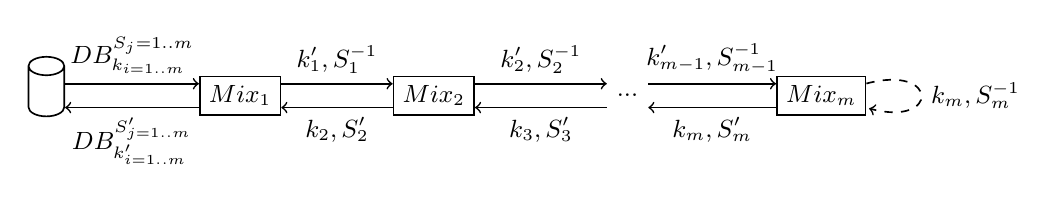
\begin{tikzpicture}[->, auto, semithick,  node distance = 7em]
\tikzstyle{every state}=[fill=white,draw=black,thick,text=black]
\node[draw, cylinder, shape border rotate=90,minimum height=5ex,minimum width=3ex]    	(0)				  {};	
\node[draw, rectangle]   		(A)[right of=0]   {\small $Mix_{1}$};
\node[draw, rectangle]    		(B)[right of=A]   {\small $Mix_{2}$};
\node[draw=none, fill=none]    		(X)[right of=B]   {\small $...$};
\node[draw, rectangle]    		(Z)[right of=X]   {\small $Mix_m$};

\path
([yshift=1ex]0.east) edge     	node{\small $DB_{k_{i=1..m}}^{S_j=1..m}$}    	([yshift=1ex]A.west)
([yshift=-1ex]A.west) edge     	node{\small $DB_{k'_{i=1..m}}^{S'_{j=1..m}}$}    	([yshift=-1ex]0.east)

([yshift=1ex]A.east) edge     	node{\small $k_1',S_1^{-1}$}    	([yshift=1ex]B.west)
([yshift=-1ex]B.west) edge     	node{\small $k_2,S_2'$}    	([yshift=-1ex]A.east)

([yshift=1ex]B.east) edge     	node{\small $k_2',S_2^{-1}$}    	([yshift=1ex]X.west)
([yshift=-1ex]X.west) edge     	node{\small $k_3,S_3'$}    	([yshift=-1ex]B.east)

([yshift=1ex]X.east) edge     	node{\small $k_{m-1}',S_{m-1}^{-1}$}    	([yshift=1ex]Z.west)
([yshift=-1ex]Z.west) edge     	node{\small $k_m,S_m'$}    	([yshift=-1ex]X.east)

(Z)    edge[loop right, dashed]    node{\small $k_m,S_m^{-1}$} (Z);

\end{tikzpicture}
\end{adjustbox}
\caption{A simple Mix-ORAM} \label{fig:ASMO}
\end{figure} 
%

\noindent\textbf{Message Format.}
In order to reduce to as much as possible the mix message size, we choose to derive the AES keys and the permutation seeds from the shared secret, $s_i$ for $mix_i$, calculated in a Diffie-Hellman assumption as in~\cite{XXXsphinx}. \iffalse\\
Let $\kappa$ be the security parameter. We call $\mathcal{G}$ a prime order cyclic group satisfying the Decisional Diffie-Hellman Assumption. $\mathcal{G}^*$ is the set of non-identity elements of $\mathcal{G}$. The element $g$ is a generator of the group, and $q$ is the prime order of $\mathcal{G}$ with $q \approx 2^{2\kappa}$.\\
We suppose each mix owns a pair of keys ($\ priv_i \in \mathbb{Z}_{q}^*$, $pub_i=g^{priv_i}\in \mathcal{G}^*$). We assume the existence of a PKI that publishes a list of all ($mix_i$,\ $pub_i$) pair.
The client randomly chooses $x\in_\mathcal{R} \mathbb{Z}_q^*$ and sends to the mix $mix_i$ the element $\alpha_i=g^{x\cdot b_i}$ with $b_i$ a binding factors, the shared secret is then $s_i=pub_i^{x\cdot b_i}$.
\fi
We finally create the AES key and the seed with the HKDF function~\cite{XXXHKDF}.
The message format is then : $${addr_{mix_i},E_{pub,\ mix_i}(s_i,\ s_i'),\ ...,\ E_{pub,\ mix_m}(s_m,\ s_m'),\ E(DB)}$$ For 128-bit security, group elements can be expressed in just 32 bytes, we have thus a maximum message size of $|addr|+2\cdot 8 \cdot 32 \cdot m + n$. 


\subsection{Parallelizing the Eviction process.}
In this section we present random transposition shuffles (RTS) and argue their use enable the eviction process to be amortized over time.
We first present the mixing time of $k$-RTS before introducing ORAM assumptions to reduce even more the expected time to achieve randomness to the eyes of the adversary.

\subsubsection{$k$-Random Transposition Shuffle.}
% Def of RTS. RTS can be broken down in independant rounds which is nice for amortization. RTS can be made oblivious by making the permutations locally. The mixing time for RTS is high, we look at oblivious k-RTS.
Random Transposition Shuffles (RTS) are widely used examples in the study of card shuffling. It consists in a player picking randomly a couple of cards from a same deck, permuting them according to a coin toss and putting them back at the same location.
These steps, usually called a round, are then repeated until the deck of cards has been properly shuffled, i.e. until every card arranging is possible.\\
We can already see why RTS are natural candidates for amortized ORAMs : if they can be broke down in independent rounds which can be spread over several entities and time, so can a randomization process based on them. Furthermore, having the client (player) permuting the data blocks (cards) locally is enough to make RTS oblivious to the eyes of an adversary.
Diaconis in 1986~\cite{aldous1986shuffling} has proved that the RTS mixing time of a deck of $n$ cards is of the order of $n\log(n)$. We thus first look at oblivious $k$-RTS, an RTS where the client picks and permutes locally $k$ distinct cards, to make the scheme more efficient.

\begin{secthm}
\textbf{Mixing time of $k$-RTS.} A $k$-random permutation shuffle of a $n$ card game reaches the uniform distribution in $\tau$ rounds, such that
\begin{align*}
E(\tau) &< \frac{2}{k}\cdot\frac{n^2}{n+1}\cdot \left ( \log(n) + \mathcal{O}(1) \right ) &\\
\sigma^2(\tau) &< \frac{4}{3} \cdot {\pi}^2 \cdot \left ( \frac{n}{k} \right )^2 &
\end{align*}
\end{secthm}

An oblivious $k$-RTS implies computation and communication cost of the order of $\mathcal{O} \left(n\cdot \log(n)\right)$.
%
\subsubsection{Oblivious Merge}
Before the eviction algorithm is run, the database can be divided in two sets of records depending on whether or not they were retrieved by the user. As such, the database can be represented as a simple binary array of $n$ bits out of which $s$ are 1s, the accessed ones, and $n-s$ are 0s, the others.
We argue that in this representation, elements of the same sets are indistinguishable to the adversary thanks to prior encryptions and permutations and thus, less rounds are necessary to correctly shuffle the database.
Indeed, this assumption significantly reduces the number of possible orderings in the adversarial view. We can prove, thanks to the Bars and Stripes theorem, that there now are ${n \choose s}$ orderings instead of $n!$.

We now consider the RTS process in that scenario and suppose the records (the bits) are re-encrypted before being permuting such that the merge of the two sets is oblivious to the adversary.

\begin{secthm}
An oblivious merge (OM) of 2 indistinguishable sets of respective size $n$ and $s$ elements requires $\tau$ rounds of 2-RTS such that any arranging is possible, with
\begin{align*}
\tau(\epsilon) &\geq \frac{1}{(\frac{n\cdot e}{s})^{\frac{s}{s-1}}-1} \log\left(\frac{1}{2 \epsilon} \right) &\\
\tau(\epsilon) &\leq \frac{n}{2\cdot s}  \cdot \left [ s \left( \log \left (\frac{n}{s}-0.5\right) +\mathcal{O}\left(1\right) \right ) - 2\log \left( 4 \cdot \epsilon\right) \right ] &\\
\end{align*}
\end{secthm}

\begin{secthm}
A $k$-oblivious Merge ($k$-OM) of 2 indistinguishable sets of respective size $n$ and $s$ requires $\tau$ rounds doing of $k$-RTS such that any arranging is possible, with
\begin{align*}
\tau(\epsilon) &\geq \frac{1}{k}  \cdot \frac{1}{(\frac{n\cdot e}{s})^{\frac{s}{s-1}}-1} \log\left(\frac{1}{2 \epsilon} \right) &\\
\tau(\epsilon) &\leq \frac{n}{2\cdot k \cdot s}  \cdot \left [ s \left( \log \left (\frac{n}{s}-0.5\right) +\mathcal{O}\left(1\right) \right ) - 2\log \left( 4 \cdot \epsilon\right) \right ] &\\
\end{align*}
\begin{proof}
We could see that the doing $k$ permutations in RTS decreased by a minimum factor of $\frac{1}{k}$, we make here the \textit{assumption} that this result is independent of the items to shuffle and is still relevant here.
\end{proof}
\end{secthm}
%
\subsubsection{Amortizable sort}
%
We now consider the mix-net as a collection of isolated mixes. When performing an eviction, we attribute to each mix  $k=\frac{n}{m}$ distinct indexes and provide them with lists of $\mathcal{O}\left ( m \cdot \log \left (\frac{n}{s} \right ) \right )$ of private and public seeds and encryption keys.\\
The unwrapping and wrapping phases consist of $r=\mathcal{O}\left ( m \cdot \log \left (\frac{n}{s} \right ) \right )$ rounds.
In the unwrapping phase as shown in the Algorithm.~\ref{alg:UAS}, the records are located in the database with the old public seeds, inversely permuted with the old private seeds and re-encrypted with the new encryption key. 
In the wrapping phase as shown in the Algorithm.~\ref{alg:WAS}, the records from the attributed section of the database are download, permuted according to the new seeds, decrypted with the old encryption keys and uploaded to the database according to the new public seeds as shown in Fig.~\ref{fig:WAS}.\\

\begin{figure}
\begin{minipage}[t]{0.475\textwidth}
\vspace{0pt}
\centering 
\begin{algorithm}[H]
\SetKwComment{Comment}{//}{}
\DontPrintSemicolon
\KwIn{Public seed $S_{pub,old,j}$;\\ \qquad Private seed $S_{prv,old,i,j}$; \\ \qquad Encryption key $Key_{new,i,j}$; \\ \qquad Number of records $k$; \\ \qquad First index $idx$;}
$Idxs \gets {\Pi}_{S_{pub,old,j}}^{-1} [idx: idx +k]$;\\
$Rcds \gets \{\}$;\\
$i\gets 0$;\\
\While{$i < k$}
{
	$Rcds.append\left (get(Idxs[i])\right)$;\\
	$i\gets i+1$;\\
}
$Rcds \gets {\Pi}_{S_{priv,old,i,j}}^{-1} \left ( Rcds \right ) $;\\
\ForAll{$r\in Rcds$}
{
	$r \gets encrypt_{Key_{new,i,j}}\left( r \right )$;
}
$put\_range \left(idx,idx+k, Rcds \right )$;\\
$\textbf{del } S_{pub,old,j},\ S_{priv,old,i,j}$;\\
\caption{Unwrapping process for the mix $i$ during round $j$}
\label{alg:UAS}
\end{algorithm}
\end{minipage}
\hfill
\begin{minipage}[t]{0.475\textwidth}
\vspace{0pt}
\centering
\begin{algorithm}[H]
\SetKwComment{Comment}{//}{}
\DontPrintSemicolon
\KwIn{Public seed $S_{pub,new,j}$;\\ \qquad Private seed $S_{prv,new,i,j}$; \\ \qquad Encryption key $Key_{old,i,j}$; \\ \qquad Number of records $k$; \\ \qquad First index $idx$;}
$Rcds \gets get\_range\left (idx,\ idx+k\right)$;\\
$Rcds \gets {\Pi}_{S_{priv,new,i,j}} \left ( Rcds \right ) $;\\
\ForAll{$r \in Rcds$}
{
	$r \gets decrypt_{Key_{old,i,j}}\left( r \right )$;
}
$Idxs \gets {\Pi}_{S_{pub,new,j}} [idx: idx +k]$;\\
$i\gets 0$;\\
\While{$i < k$}
{
	$put\left( Idxs[i],\ Rcds[i] \right )$;\\
	$i\gets i+1$;
}
$\textbf{del } Key_{old,i,j}$;\\
\caption{Wrapping process for the mix $i$ during round $j$}
\label{alg:WAS}
\end{algorithm}
\end{minipage}
\caption{Amortizable sort, wrapping and unwrapping algorithms.}
\end{figure}


\begin{figure}
\centering
\begin{minipage}[t]{0.45\textwidth}
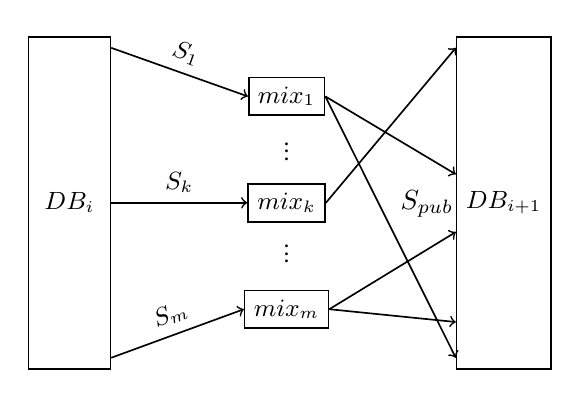
\begin{tikzpicture}[->,
auto,
semithick, 
scale=0.5,
block/.style={draw, fill=white, rectangle, font=\small}]


\node[block, anchor = west, minimum height=12em, minimum width={width("$DB_{i+1}$")}] 		(0)		{$DB_i$};

\node[block]				(B)[right of=0, xshift=5em]		{$mix_k$};
\node[draw=none, fill=none]    		(X)[above of=B, yshift=-1em]		  [rotate=-90]{...};
\node[draw=none, fill=none,]    		(Y)[below of=B, yshift=1em]		  [rotate=-90]{...};
\node[block, anchor= north]		(A)[above of=B, yshift=1em]		{$mix_1$};
\node[block, anchor = south]		(C)[below of=B, yshift=-1em]		{$mix_m$};

\node[block, anchor = east, minimum height=12em]		(1)[right of=B, xshift = 5em]		{$DB_{i+1}$};


\path[->, midway]
 ([yshift=-2ex]0.north east) edge node[sloped, above]{\small $S_1$} (A.west)
 (0) edge node[sloped, above]{\small $S_k$} (B.west)
 ([yshift=2ex]0.south east) edge node[sloped, above]{\small $S_m$} (C.west)

 (A.east) edge node[above,yshift=4ex]	{} 			(1)
 (A.east) edge node			{$S_{pub}$} 			([yshift=2ex]1.south west)
 (B.east) edge node			{} 	([yshift=-2ex]1.north west)
 (C.east) edge node			{} 			([yshift=8ex]1.south west)
 (C.east) edge node			{} 			(1);
 
\end{tikzpicture}
\caption{Wrapping in a round of Amortizable sort} \label{fig:WAS}
\end{minipage}
\hfill
\begin{minipage}[t]{0.45\textwidth}
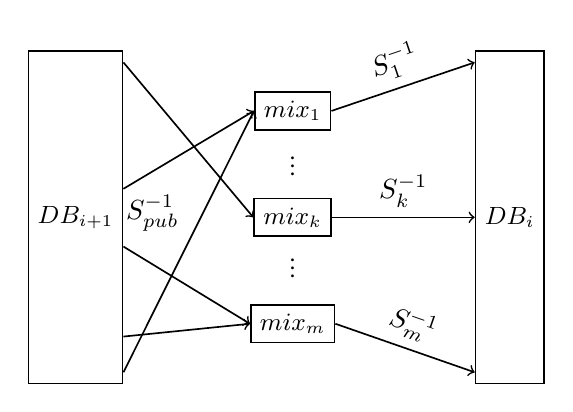
\begin{tikzpicture}[->,
auto,
semithick, 
scale=0.5,
block/.style={draw, fill=white, rectangle, font=\small}]


\node[block, anchor = west, minimum height=12em, minimum width={width("$DB_{i+1}$")}] 		(0)		{$DB_{i+1}$};

\node[block]				(B)[right of=0, xshift=5em]		{$mix_k$};
\node[draw=none, fill=none]    		(X)[above of=B, yshift=-1em]		  [rotate=-90]{...};
\node[draw=none, fill=none,]    		(Y)[below of=B, yshift=1em]		  [rotate=-90]{...};
\node[block, anchor= north]		(A)[above of=B, yshift=1em]		{$mix_1$};
\node[block, anchor = south]		(C)[below of=B, yshift=-1em]		{$mix_m$};

\node[block, anchor = east, minimum height=12em]		(1)[right of=B, xshift = 5em]		{$DB_{i}$};


\path[->, midway]
 (0) 							edge node		{} 		(A.west)
 ([yshift=2ex]0.south east) 		edge node		{$S_{pub}^{-1}$} 		(A.west)
 ([yshift=-2ex]0.north east)		edge node		{} 		(B.west)
 ([yshift=8ex]0.south east) 		edge node		{} 		(C.west)
 (0)						 		edge node		{} 		(C.west)

 (A.east) edge node[sloped, above]			{$S_1^{-1}$} 			([yshift=-2ex]1.north west)
 (B.east) edge node[sloped, above]			{$S_k^{-1}$} 			(1)
 (C.east) edge node[sloped, above]			{$S_m^{-1}$} 			([yshift=2ex]1.south west);
 
\end{tikzpicture}
\caption{Unwrapping in a round of Amortizable sort} \label{fig:WAS}
\end{minipage}
\caption{Wrapping and corresponding unwrapping.}
\end{figure} 

\subsection{Parallel Mix-ORAM}
\todo{eviction as in 3.2.3, new lookup, message format... }

The client thus provides to each mix the $index$ and range $k=\frac{n}{m}$ for the record allocation, $ \frac{3}{2} \cdot m \cdot \log \left (\frac{n}{s} \right ) $ seeds in total and $ m \cdot \log \left (\frac{n}{s} \right )$ encryption keys and store in total $\mathcal{O}\left (m \cdot \log \left (\frac{n}{s}  \right) \right )$ bits. To find the ORAM index of a precise record, the client performs the index lookup function written in Algorithm.~\ref{alg:IAS}.

\begin{algorithm}
\SetKwComment{Comment}{//}{}
\DontPrintSemicolon
\KwIn{Seeds $new\_S_{pub},\ new\_S_{prv}$; \\ \qquad Total number of records $n$; \\ \qquad Number of mixes $n$;\\ \qquad number of rounds $r$;\\ \qquad Index to retrieve $index$;}
$k \gets \frac{n}{m}$;\\
$i \gets 0$;\\
\While{$i < r$}
{
	$mix \gets \frac{index}{k} $;\\
	$subindex \gets index\ \%\ k$;\\
	$subindex \gets {\Pi}_new\_S_{prv, mix, i}(subindex) * $;\\
	$index \gets {\Pi}_new\_S_{pub,j}(k*mix+subindex) *$;\\
	$i\gets i+1$;
}
\KwOut{$index$}
* These steps were simplified for easier reading.\\
\caption{Index Lookup}
\label{alg:IAS}
\end{algorithm}

\noindent\textbf{Message Format.}
In order to reduce to as much as possible the mix message size, we choose to derive the AES keys and the permutation seeds from the shared secret, $s_i$ for $mix_i$, calculated in a Diffie-Hellman assumption as in~\cite{XXXsphinx}. \iffalse\\
Let $\kappa$ be the security parameter. We call $\mathcal{G}$ a prime order cyclic group satisfying the Decisional Diffie-Hellman Assumption. $\mathcal{G}^*$ is the set of non-identity elements of $\mathcal{G}$. The element $g$ is a generator of the group, and $q$ is the prime order of $\mathcal{G}$ with $q \approx 2^{2\kappa}$.\\
We suppose each mix owns a pair of keys ($\ priv_i \in \mathbb{Z}_{q}^*$, $pub_i=g^{priv_i}\in \mathcal{G}^*$). We assume the existence of a PKI that publishes a list of all ($mix_i$,\ $pub_i$) pair.
The client randomly chooses $x\in_\mathcal{R} \mathbb{Z}_q^*$ and sends to the mix $mix_i$ the element $\alpha_i=g^{x\cdot b_i}$ with $b_i$ a binding factors, the shared secret is then $s_i=pub_i^{x\cdot b_i}$.
\fi
We create the AES key and the private seed with the HKDF function~\cite{XXXHKDF}. The public seed is created by the user.
The message format is then : $${addr_{mix_i},E_{pub,\ mix_i}(S_{pub},\ s_i),\ records}$$ For 128-bit security, group elements can be expressed in just 32 bytes, we have thus a maximum message size of $|addr|+2\cdot 8 \cdot 32 + n$. 


\subsection{Lowering Eviction Costs}

In order to lower the eviction costs sustained by the mix-net, optimizations on each side of the channel can be done.

\raphael{Differentially private oblivious shuffle}

\section{Evaluation}
\subsection{Implementation and Benchmark}
\subsection{Performances}
\subsection{Comparison}

\section{Discussion}
\label{Discussion}

\subsection{Active Adversary}
Randomized Partial Checking
Reputation system

\subsection{Lowering the eviction costs through the access method}

\noindent\textbf{Changing the access method.}The client, to lower the eviction costs, could instead of fetching only the requested record query retrieve $k-1$ other dummy records and permuting all of them before updating them back to the ORAM.
Doing so, we can progress further towards the uniform distribution before the eviction process, measure the distance between the two distributions and reduce the database shuffling cost by having the mix-net performing cheaper and weaker permutations.
What's more, requesting more records, and doing so on different servers, can help in hiding the access pattern as discussed in~\cite{toledo2016lower}.\\

\noindent\textbf{Considering fake access.} When a user wants to access a record which already is in the stash, a random database access is performed to hide potential frequency attacks: an adversary having observed the record access frequency beforehand and knowing the average access per day would be able to guess which records are in the stash by not observing accesses which should happen.
These fake accesses can be considered as free permutations as no fetched records need to remain in the stash, thus we can arbitrarily set $k_{in}=k_{out}$.\\

\begin{secthm}
In the case of a uniform distribution access we have an average number 0 of fake access for $s<<n$.\\
\end{secthm}

However it is well known that the frequency access of records is not uniform, in that case we can count a strictly positive number of fake accesses.
\begin{secthm}
Let $A$ be the access distribution. Let's call $v_0$ and $v_1$ the volume above the line $y=0$ and under it respectively.
The average number of fake access is $ \frac{v0}{v1}$.
\begin{proof}
 The volume under such line represents the number of real accesses a user does while the volume above it represents accesses in the stash which leads to fake accesses.
 When the number of accesses is great, the access frequency approaches the average number of accesses.
\end{proof}
\end{secthm}

\noindent\textbf{Delaying the eviction.} When querying an item, in the Square Root solution, the user writes in the stash the retrieved record and put at its location in the database a dummy. Instead of writing dummies in the database, the client could write records from the stash and put at their location dummies. In that case, the size of the stash doesn't increase and we can delay even more the eviction process.


\section{Acknowledgement}
Danezis was supported by H2020  PANORAMIX Grant (ref. 653497) and EPSRC Grant EP/M013286/1; and Toledo by Microsoft Research.


\section{Conclusion}
\label{Conclusion}
\begin{itemize}
 \item New ORAM with mix-net
 \item amortizable eviction
 \item can fetch while eviction running
 \item multi-user friendly as all the secrets are on the server
\end{itemize}

\bibliography{mix_oram}
\bibliographystyle{splncs03}

\section{Appendix}
\subsection{Proof $k$-RTS}
\begin{proof}
To first prove the upper bound and variance, we use Diaconis et al. results~\cite{aldous1986shuffling} which states that $\tau$ defined in the following game is a strong stationary time.
In a random transposition shuffle, the cards chosen by the right and left hands at time $t$ are respectively called $R_t$ and $L_t$. Assuming that when $t=0$, no card is marked, we mark $R_t$ if
$R_t$ was unmarked before and either $L_t$ is marked or $L_t = R_t$. The variable $\tau$ represents the time when every card has been marked, we call it the stopping time.

Let be $\tau_t$ the number of transpositions after the $t^{th}$ card is marked, up to and including when the $(t+1)^{th}$ is marked. $$\tau = \sum_{i=0}^{n-1} \tau_i$$.
The $\tau_t$ are independent geometric variables with probability of success $p_t$ as implied by the game rules.
The probability of success corresponds to the probability of marking at least one card, one to $t$ cards exactly. To do so, the right cards must be chosen from the unmarked set, comprising $n-t$ cards at time $t$,
and the left cards from the union of the marked set and the right cards.
\begin{align*}
 p_t &= \sum_{i=1}^{min(k,n-t)} {k \choose i} \cdot {t+1 \choose i} \cdot {n-t \choose i}\cdot{n \choose i}^{-2}&\\
 &= k \frac{(t+1)\cdot(n-t)}{n^2} + \alpha_{n,t,k},\ 0 < \alpha_{n,t,k} = \mathcal{O}\left(n^{-k}\right )
\end{align*}

We can thus rewrite $\tau$'s expectation as following.
\begin{align*}
 E(\tau) &= \sum_{t=0}^{n-1} \frac{1}{p_{t}} = \sum_{t=0}^{n-1} \frac{n^2}{k \cdot (t+1)\cdot(n-t) + \frac{\alpha_{n,t,k}}{n^2}}&\\
 &< \sum_{t=0}^{n-1} \frac{n^2}{k \cdot (t+1)\cdot(n-t)}  &\\
 &< \frac{1}{k} \cdot \frac{n^2}{n+1} \cdot  \sum_{t=0}^{n-1} \left ( \frac{1}{t+1} + \frac{1}{n-t} \right ) &\\
% &< \frac{2}{k} \cdot \frac{n^2}{n+1} \cdot H_n  \\
 &< \frac{2}{k} \cdot \frac{n^2}{n+1} \cdot \left( \ln(n) + \gamma +\mathcal{O}(\frac{1}{n}) \right), \gamma = \lim_{n \to \infty} H_n - \ln(n)& \\
 \end{align*}
 \begin{align*}
 var(\tau) &= \sum_{t=0}^{n-1}\frac{1-p_t}{{p_t}^2}\ <\  \sum_{t=0}^{n-1}\frac{1}{{p_t}^2} &\\
 &< \sum_{t=0}^{n-1}\frac{1}{\left ( k \frac{(t+1)\cdot(n-t)}{n^2} + \alpha_{n,t,k}\right )^2}\\\
 &<\ \sum_{t=0}^{n-1} \frac{1 }{\left ( k \frac{(t+1)\cdot(n-t)}{n^2} \right )^2} &\\
 %&< \frac{n^4}{k^2} \left ( \sum_{t=0}^{\frac{n}{2}-1} \frac{1}{\left ( (t+1)(n-t)\right )^2}  + \sum_{t=\frac{n}{2}}^{n-1} \frac{1}{\left ( (t+1)(n-t)\right )^2} \right ) &\\
 &< 2 \cdot \left (\frac{n}{k} \right )^2 \cdot \left (\frac{n}{n/2} \right )^2 \cdot \sum_{t=0}^{n/2-1} \frac{1}{(t+1)^2} &\\
 &< \frac{4}{3} \pi^2 \cdot \left (\frac{n}{k} \right )^2 
\end{align*}
\\

To now prove the lower bound of $\tau$, we will compare the number of fixed points of a permutation $\sigma$, $F(\sigma)$, for our shuffle, the permutation
obtained from the identity by applying $kt$ random transpositions $ P^{kt}(id, \cdot)$, and the uniform distribution $\pi$, or more precisely compare the corresponding probabilities over the set $A=\{\sigma : F(\sigma) \geq \frac{\mu}{2} \}$.
We can say that after $t$ shuffles, the number of untouched cards of our shuffle has the same distribution as the number $R_{2kt}$ of uncollected coupon types after $2kt$ steps of a coupon collector chain
and that about $ P^{kt}(id, \cdot)$ that the associate $F(\sigma)$ is at least as large as the number of cards that were touched by none of the transpositions, i.e. $P^{kt}(id,A) \geq P(R_{kt}\geq A) $.

We know that the $R_{2kt}$ has expectation $\mu = np$  with $p=\left ( 1 - \frac{1}{n} \right )^{2kt}$, variance $var = np(1-p) <\mu$ and by Chebyshev, we know that $\Pr(R_{2kt}\leq \frac{\mu}{2})\leq \frac{4}{\mu}$
as $\Pr(|R_{2kt} - \mu|\geq \frac{\mu}{2}) = \Pr(R_{2kt} \geq \frac{3\mu}{2}) + \Pr(R_{2kt} \leq \frac{\mu}{2}) > \Pr(R_{2kt} \leq \frac{\mu}{2})$.\\

By Markov's inequality we know that $\pi(A) \leq \frac{2}{\mu}$.\\

As $P^{kt}(id,A) \geq P(R_{kt}\geq A) $, we also have $P^{kt}(id,A^c) \leq P(R_{2kt}\leq A) \leq \frac{4}{\mu} $ which leads to $P^{kt}(id,A)\geq1 - \frac{4}{\mu}$.\\

Thus we have $d(t)=||P^{kt}(id,) - \pi ||_{TV} \geq |1 - \frac{4}{\mu} - \frac{2}{\mu}| \geq 1 - \frac{6}{\mu}$.\\

We want to find the minimum $t$ such that $1-\frac{6}{\mu}\geq \epsilon$, which is equivalent to $n \cdot \left ( 1 - \frac{1}{n} \right )^{2kt} \geq \frac{6}{1-\epsilon}$ and to
$$\log\left(\frac{n\cdot (1-\epsilon)}{6}\right) \geq 2\cdot k\cdot t \cdot \log \left ( \frac{n}{n-1} \right )$$
As $\log(1+x) \leq x$, the previous inequality holds if $\log\left(\frac{n\cdot (1-\epsilon)}{6}\right) \geq   \frac{2kt}{n-1} $ which means that if $t\leq \frac{n-1}{2k}\cdot \log\left ( \frac{n(1-\epsilon)}{6}\right )$ then $d(t)\geq \epsilon$.
Thus,
$$\tau \left (\epsilon \right ) \geq \frac{n-1}{2k} \ln(n\cdot \frac{1-\epsilon}{6}) $$.
\end{proof}

\subsection{Proof of Oblivious Merge}
\begin{proof}
We want to find the mixing time $\tau(\epsilon)$ of our oblivious merge of two sets of indistinguishable elements. To do so, we use the bound of the mixing time of an irreducible ergodic Markov Chain, where $p = \frac{1}{|V|}$ and $1-\lambda^*$ is the spectral gap,
$$\frac{\lambda^*}{1-\lambda^*} \cdot \log\left(\frac{1}{2 \epsilon} \right)\leq \tau(\epsilon) \leq \frac{1}{1-\lambda^*}\cdot \log \left( \frac{1}{2 \epsilon \cdot \sqrt{p}}\right) $$

We now want to find a bound for $\lambda^*$. We represent the arranging of merge of the 2 distinct sets by the graph $\mathcal{G}$, a $k$-regular graph with $v$ vertices corresponding to the different orderings and the undirected edges to transpositions of two elements.
By definition, the eigenvalues of the transition matrix of the $\mathcal{G}$ are $k={\lambda'}_0 > {\lambda'}_1 \geq  ... \geq {\lambda'}_{n-1}$, and we have,
$$\text{diam}\left( \mathcal{G}\right) \leq \frac{log(v-1)}{log(\frac{k}{{\lambda'}^*})}+1 \text{ with } {\lambda'}^* = max_{i\neq0}({\lambda'}_i)= k \cdot \lambda^*$$
with $diam\left( \mathcal{G} \right)=s$ the diameter of the graph, $v= {n \choose s}$ the number of vertices and $k=s\cdot(n-s)$.\\


We can thus find a first relation:
\begin{align*}
log(\frac{k}{{\lambda'}^*}) &= log(\frac{1}{{\lambda}^*}) \leq\frac{\log(v-1)}{\text{diam}\left(\mathcal{G}\right)-1}&\\
log({{\lambda}^*}) &\geq  \frac{log(v-1)}{1-\text{diam}\left(\mathcal{G}\right)}&\\
{\lambda}^* &\geq (v-1)^{\frac{-1}{\text{diam}\left(\mathcal{G}\right)-1}}\\
{\lambda}^* &\geq \left ({n \choose s}-1 \right )^{\frac{1}{1-s}} \geq \left (\frac{n\cdot e}{s} \right )^{\frac{s}{1-s}}
\end{align*}

And can derive the minimum value of $\Delta=\frac{\lambda^*}{1-\lambda^*}$,
\begin{align*}
 \Delta &= \frac{1}{\left (\lambda^*\right )^{-1}-1}\\
 &\geq \frac{1}{\left (\frac{n \cdot e }{s} \right )^{\frac{s}{s-1}}-1}\\
\end{align*}


To find an upper-bound of $\lambda^*$, we will focus on the spectral gap bounding.
Let's $\mathcal{G}_{0,1}=\{0,1\}^n$ be the group of elements with the XOR operation and $\mathcal{S}=\{x \in \mathcal{G},\ weight(x)=s\}$ the symmetric subset of $\mathcal{G}$ of n-binary array with $s$ 1s and $n-s$ 0s.
We call $Cay_{n,s}=Graph\left(  \mathcal{G}_{0,1}, \mathcal{S} \right) $ the Cayley graph generated from these structures.

\begin{lemma}
Let $\mathcal{G}$ be a finite Abelian group, $\chi\ :\  \mathcal{G} \rightarrow \mathbb{C}$ be a character of $\mathcal{G}$, $\mathcal{S} \subseteq \mathcal{G}$ be a symmetric set.
Let $M$ be the normalized adjacency matrix of the Cayley graph $G = Cay(\mathcal{G},\mathcal{S})$.
Consider the vector $x \in \mathbb{C}^\mathcal{G}$ such that $x_a = \chi(a)$. Then x is an eigenvector of $G$, with eigenvalue $$ \frac{1}{\mathcal{S}} \sum_{s\in \mathcal{S}} \chi\left(s\right)$$
\end{lemma}

\begin{theorem}
The Cayley graph $Cay_{n,s}$ has for eigenvalues $\mu_0 = 1 > \mu_1 \geq ... \geq \mu_n$ with, 
$$\mu_r = \frac{1}{\left | \mathcal{S} \right |} \sum_{i=1}^{min(r, n-r)} \left ( -1 \right )^i {r \choose i}{n-r \choose s-i}\\$$
\end{theorem}

\begin{subproof}
$\forall r \in \{0,1\}^n$, with $\chi_r(x)=\left ( -1 \right )^{\sum r_i \cdot x_i}$, we have,
\begin{align*}
\mu_r &= \frac{1}{\mathcal{S}} \sum_{s\in \mathcal{S}} \chi\left(s\right) \\
&= \frac{1}{\left | \mathcal{S} \right |} \sum_{s\in \mathcal{S}} \left ( -1 \right )^{\sum r_i \cdot s_i} \\
&=  \frac{1}{\left | \mathcal{S} \right |} \left ( \left | ``1" \right | - \left | ``-1"  \right| \right ) \\
&= \frac{1}{\left | \mathcal{S} \right |} \sum_{i=1}^{min(r, s)} \left ( -1 \right )^i {r \choose i}{n-r \choose s-i} \\
&= 1 - \frac{2}{{n \choose s}} \cdot \sum_{i=0}^{min(\frac{r-1}{2}, \frac{s-1}{2})} {r \choose 1+2i}{n-r \choose s-2i-1} \\
&= \frac{{n-r \choose s}}{{n \choose s}} \ _2F_1(-r,-s,n-2r+1,-1)
%&= \frac{1}{\left | \mathcal{S} \right |} \left [ \sum_{i=0}^{min(\frac{r}{2},\frac{n-r}{2})} {r \choose 2i}{n-r \choose s-2i} - \sum_{i=0}^{min(\frac{r-1}{2}, \frac{n-r-1}{2})} {r \choose 1+2i}{n-r \choose s-2i-1}\right] 
\end{align*}
\end{subproof}


Remark. We recognize here the Vandermonde identity with alternating numbers. We argue that the eigenvalues of the Cayley graph $Cay_{n,s}$ are all positive as the smallest eigenvalue is null.
For $r=n-r$, the expression simplifies to $\mu_r = {r \choose \frac{n}{2}}$ if $n$ even, 0 otherwise.
For $r=1$, the expression simplifies to $\mu_1 = 1 - 2\cdot \frac{s}{n}$, the spectral gap of $Cay_{n,s}$ is thus equal to $2\cdot \frac{s}{n}$.\\\

We notice that the first graph $\mathcal{G}$ actually is a sub-graph of $Cay_{n,s}$ and as such the the adjacent matrix of the first graph is included in the second's.
For $s>1$, $Cay_{n,s}$ is divided in two sub-graphs representing the cosets of $\{0,1\}^n$ as $\mathcal{S}$ is not a generating group of $\mathcal{G}_{0,1}$, $\mathcal{G}$ is only contained in one of the sub-graphs.
We use the Cauchy's Interlace Theorem to bound the eigenvalues of $\mathcal{G}$ with the ones of $Cay_{n,s}$,.

\begin{theorem}
Let $M$ be a Hermitian $n \times n$ matrix with eigenvalues ${\mu'}_0\geq ... \geq {\mu'}_{n-1}$ and $N$ a $m \times m$ sub-matrix of $M$ with eigenvalues ${\lambda'}_0\geq ... \geq {\lambda'}_{m-1}$ , we have
$$ {\mu'}_i \geq {\lambda'}_i \geq {\mu'}_{n-m+i+1} $$
\end{theorem}

We are here only interested in an upper-bound of $\lambda*$, as we have $\mu_{2^n+2-{n \choose s}}\leq \lambda_1\leq 1-2\frac{s}{n}$ and $0 \leq \lambda_n \leq \mu_2$, $\lambda* \leq 1-2\frac{s}{n}$. We thus have $\frac{1}{1-\lambda*}\leq\frac{n}{2\cdot s}$
\end{proof}

\subsection{Proof of Fake access}
\begin{proof}
 We want to prove that the average number of fake access is 0 in case of a uniform distribution. To do so, we consider the Markov chain and its Transition Matrix.
 The transition matrix $P$ represents the $s$ transient state, in which the stash is not completely filled, and the absorption state in which the stash is full.
Thus, $P$ can be decomposed in 4 sub-matrices: the square sub-matrix $Q_s$ representing all the transient state, the column matrix R with the probabilities of transitioning to the absorbing state, the null row matrix and the absorption matrix.
\[
\begin{bmatrix}
   Q_s & R \\
   0_{1\times s}   & I_1 \\
\end{bmatrix}
\]
To find the average number of steps from one state to the absorbing one, we have solve the following equation, each row corresponding to the average number of steps from the corresponding state (the stashed filled with some records) to the state where the stash is full.
\begin{align*}
 t &= \left (\sum_{k=0}^{\infty} {Q_s}^k \right ) 1 \\
   &= (I_s -Q_s )^{-1} 1
\end{align*}
This equation has a solution since $M=I_s -Q_s$ have independent rows and thus an inverse that we call $N$.
By calculus we find that,
\begin{align*}
 n_{i,j} &= 0 &\text{ if } i>j,\\ 
 n_{i,j} &= \frac{1}{m_{i,i}} &\text{ if } i=j,\\
 n_{i,j} &= - n_{i+1,j } \cdot \frac{m_{i,i+1}}{m_{i,i}} &\text{ if } i<j 
\end{align*}
which can be simplified by
\begin{align*}
 n_{i,j} &= 0 &\text{ if } i>j,\\ 
 n_{i,j} &= \frac{1}{m_{j,j}} \prod_{k=1}^{j-1} \left ( - \frac{m_{i,k+1}}{m_{k,k}}\right ) &\text{ if } i\leq j
\end{align*}
We only want to calculate the first solution $S_1$ from the equation.
\begin{align*}
 S_1 &= \sum_{j=0}^{s-1} \frac{1}{m_{j,j}} \prod_{k=1}^{j-1} \left ( - \frac{m_{i,k+1}}{m_{k,k}}\right ) \\
     &= \sum_{j=1}^{s-1} \frac{1}{m_{j,j}} \text{ as } m_{i,k+1}= -m_{k,k} \\
     &= \sum_{j=0}^{s-1} \frac{1}{1-\frac{j}{n}} = \sum_{j=0}^{s-1} \left (1 + \frac{j}{n-j} \right ) \\
     &= s + \sum_{j=0}^{s-1} \frac{j}{n-j} \\   
\end{align*}
As $s$ steps are required to fill the stash, we thus find the following inequality for the number of fake access $f$:
$$ \frac{s \cdot (s+1)}{2 \cdot n} < f < \frac{s \cdot (s+1)}{2 \cdot (n+1-s)} $$
\end{proof}


\end{document}
